\section{Full Evaluation Tables}
\label{app:eval}

We give the full per-domain, per-strategy, and per-difficulty
breakdowns referenced in Section~\ref{sec:eval}, plus the cost ledger
and the post-evaluation zero-correct audit.

\begin{table}[h]
  \centering
  \footnotesize
  \caption{Per-config per-domain accuracy (\%).}
  \label{tab:full-domain}
  \begin{tabular}{lrrrrrr}
    \toprule
    Config & Regions & Varieties & Producers & Viticulture & Winemaking & Business \\
    \midrule
    claude-opus-4.7              & 83.2 & 80.2 & 86.8 & 77.9 & 86.6 & 64.2 \\
    claude-haiku-4.5             & 55.8 & 49.7 & 58.7 & 54.2 & 56.7 & 37.8 \\
    gpt-5                        & 88.1 & 78.2 & 88.4 & 82.8 & 80.7 & 63.0 \\
    gpt-5-mini                   & 82.1 & 74.4 & 83.5 & 77.5 & 77.5 & 66.3 \\
    gemini-2.5-pro               & 87.0 & 78.8 & 89.0 & 78.5 & 77.5 & 61.8 \\
    gemini-2.5-flash             & 76.9 & 72.9 & 82.3 & 73.6 & 77.5 & 60.6 \\
    llama-3.3-70b                & 68.9 & 62.9 & 77.2 & 65.7 & 70.6 & 50.4 \\
    llama-3.1-8b                 & 62.2 & 55.6 & 69.5 & 61.7 & 59.4 & 47.6 \\
    deepseek-v3                  & 74.4 & 68.5 & 73.2 & 70.8 & 69.0 & 51.2 \\
    qwen-2.5-72b                 & 69.0 & 65.1 & 73.4 & 67.5 & 70.1 & 52.8 \\
    qwen-2.5-7b                  & 59.1 & 55.6 & 59.4 & 57.4 & 57.8 & 44.7 \\
    mistral-large-2411           & 71.5 & 65.6 & 75.4 & 69.4 & 73.3 & 51.6 \\
    o3                           & 88.4 & 81.3 & 90.9 & 80.3 & 76.5 & 65.4 \\
    gemini-2.5-pro-thinking      & 86.5 & 80.5 & 90.0 & 80.5 & 83.4 & 60.2 \\
    deepseek-r1                  & 80.5 & 73.6 & 85.6 & 72.2 & 76.5 & 64.6 \\
    claude-opus-4.7-thinking     & 83.2 & 80.9 & 87.0 & 78.7 & 84.0 & 61.4 \\
    \midrule
    \textbf{Mean (16 configs)}   & \textbf{76.0} & \textbf{70.2} & \textbf{79.4} & \textbf{71.8} & \textbf{73.6} & \textbf{56.5} \\
    \bottomrule
  \end{tabular}
\end{table}

\begin{figure}[h]
  \centering
  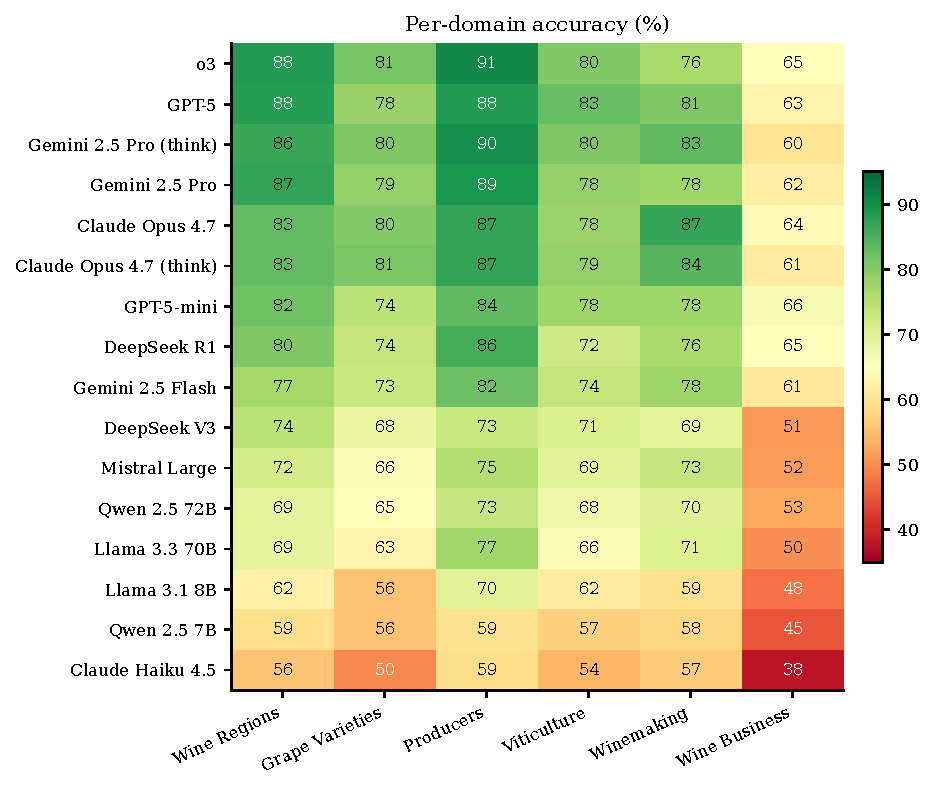
\includegraphics[width=0.78\linewidth]{figures/fig_domain_heatmap.pdf}
  \caption{Per-domain accuracy as a heatmap. \emph{Wine business} is
    the hardest domain across every tier (mean 56.5\%) — both because
    business-domain facts are sparser in the training distribution and
    because the C4 difficulty re-label promoted business questions
    that are computationally harder (multi-fact reasoning over
    regulation).}
  \label{fig:domain-heatmap}
\end{figure}

\begin{table}[h]
  \centering
  \footnotesize
  \caption{Per-config per-strategy accuracy (\%).}
  \label{tab:full-strategy}
  \begin{tabular}{lrrrrr}
    \toprule
    Config & FTQ & Scenario & Template & Comparative & Distractor \\
    \midrule
    claude-opus-4.7              & 77.7 & 85.6 & 92.8 & 79.5 & 82.7 \\
    claude-haiku-4.5             & 47.5 & 62.7 & 70.7 & 53.3 & 56.8 \\
    gpt-5                        & 79.9 & 80.9 & 95.4 & 79.5 & 87.9 \\
    gpt-5-mini                   & 73.8 & 80.6 & 92.8 & 78.3 & 84.7 \\
    gemini-2.5-pro               & 77.4 & 87.5 & 93.1 & 82.4 & 86.4 \\
    gemini-2.5-flash             & 69.5 & 84.0 & 89.7 & 77.5 & 79.5 \\
    llama-3.3-70b                & 59.5 & 80.6 & 89.7 & 64.8 & 71.9 \\
    llama-3.1-8b                 & 52.2 & 70.5 & 89.7 & 60.2 & 63.7 \\
    deepseek-v3                  & 64.5 & 80.3 & 86.4 & 71.7 & 73.3 \\
    qwen-2.5-72b                 & 59.6 & 79.3 & 88.7 & 69.3 & 73.6 \\
    qwen-2.5-7b                  & 49.1 & 72.1 & 78.9 & 57.0 & 61.0 \\
    mistral-large-2411           & 62.7 & 80.6 & 87.4 & 67.6 & 73.3 \\
    o3                           & 79.9 & 84.3 & 94.9 & 84.8 & 88.4 \\
    gemini-2.5-pro-thinking      & 78.5 & 88.4 & 95.6 & 84.0 & 84.2 \\
    deepseek-r1                  & 73.4 & 75.5 & 92.5 & 77.0 & 80.7 \\
    claude-opus-4.7-thinking     & 77.3 & 85.6 & 93.6 & 80.3 & 83.0 \\
    \midrule
    \textbf{Mean (16 configs)}   & \textbf{67.6} & \textbf{79.9} & \textbf{89.5} & \textbf{73.0} & \textbf{76.9} \\
    \bottomrule
  \end{tabular}
\end{table}

\begin{figure}[h]
  \centering
  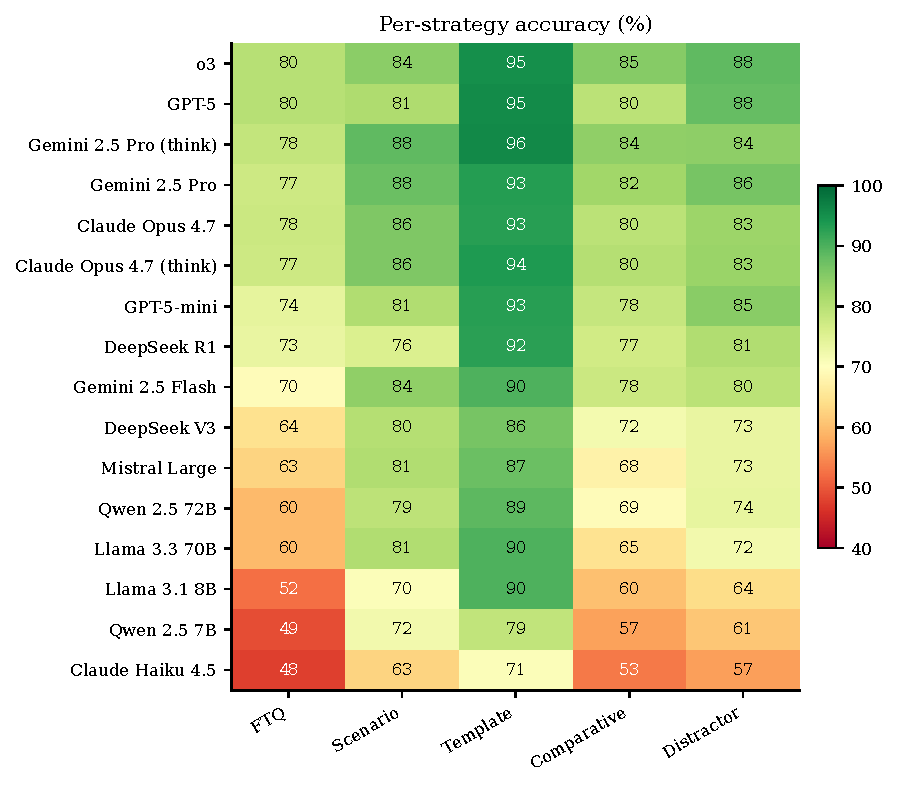
\includegraphics[width=0.7\linewidth]{figures/fig_strategy_heatmap.pdf}
  \caption{Per-strategy accuracy heatmap. Templates are the easiest
    strategy uniformly (89.5\% mean), even for small models, because
    they are deterministic single-fact recall questions. The
    fact-to-question strategy is hardest because its distractors are
    sampled from confusable same-category entities; comparative
    questions add the constraint that the model must integrate two
    facts.}
  \label{fig:strategy-heatmap}
\end{figure}

\begin{table}[h]
  \centering
  \footnotesize
  \caption{Per-config per-difficulty accuracy (\%).}
  \label{tab:full-difficulty}
  \begin{tabular}{lrrrr}
    \toprule
    Config & L1 (entry) & L2 & L3 & L4 (expert) \\
    \midrule
    claude-opus-4.7              & 98.0 & 77.0 & 86.7 & 69.1 \\
    claude-haiku-4.5             & 74.3 & 48.3 & 59.9 & 38.8 \\
    gpt-5                        & 98.3 & 82.4 & 87.5 & 69.2 \\
    gpt-5-mini                   & 98.0 & 73.7 & 84.7 & 64.8 \\
    gemini-2.5-pro               & 98.6 & 79.2 & 87.3 & 68.5 \\
    gemini-2.5-flash             & 95.4 & 70.9 & 82.2 & 60.1 \\
    llama-3.3-70b                & 91.9 & 60.6 & 74.8 & 50.3 \\
    llama-3.1-8b                 & 84.8 & 55.4 & 65.3 & 45.0 \\
    deepseek-v3                  & 95.8 & 65.9 & 76.3 & 52.4 \\
    qwen-2.5-72b                 & 93.2 & 60.5 & 73.7 & 51.4 \\
    qwen-2.5-7b                  & 82.0 & 50.6 & 60.0 & 43.3 \\
    mistral-large-2411           & 94.4 & 63.1 & 73.3 & 54.0 \\
    o3                           & 98.4 & 81.4 & 89.4 & 71.2 \\
    gemini-2.5-pro-thinking      & 99.1 & 80.2 & 88.3 & 69.4 \\
    deepseek-r1                  & 97.5 & 74.2 & 82.0 & 62.1 \\
    claude-opus-4.7-thinking     & 98.3 & 76.8 & 87.0 & 68.6 \\
    \midrule
    \textbf{Mean (16 configs)}   & \textbf{93.6} & \textbf{68.8} & \textbf{78.7} & \textbf{58.7} \\
    \bottomrule
  \end{tabular}
\end{table}

\begin{table}[h]
  \centering
  \footnotesize
  \caption{Reasoning lift per difficulty tier ($\delta$ = thinking $-$ standard, pp).}
  \label{tab:reasoning-by-diff}
  \begin{tabular}{lrrrr}
    \toprule
    Pair & L1 & L2 & L3 & L4 \\
    \midrule
    Claude Opus 4.7 (think vs std)        & $+$0.3 & $-$0.2 & $+$0.3 & $-$0.5 \\
    Gemini 2.5 Pro (think vs std)         & $+$0.5 & $+$1.0 & $+$1.0 & $+$0.9 \\
    OpenAI o3 vs GPT-5                    & $+$0.1 & $-$1.0 & $+$1.9 & $+$2.0 \\
    DeepSeek R1 vs V3                     & $+$1.7 & $+$8.3 & $+$5.7 & $+$9.7 \\
    \bottomrule
  \end{tabular}
\end{table}

\begin{figure}[h]
  \centering
  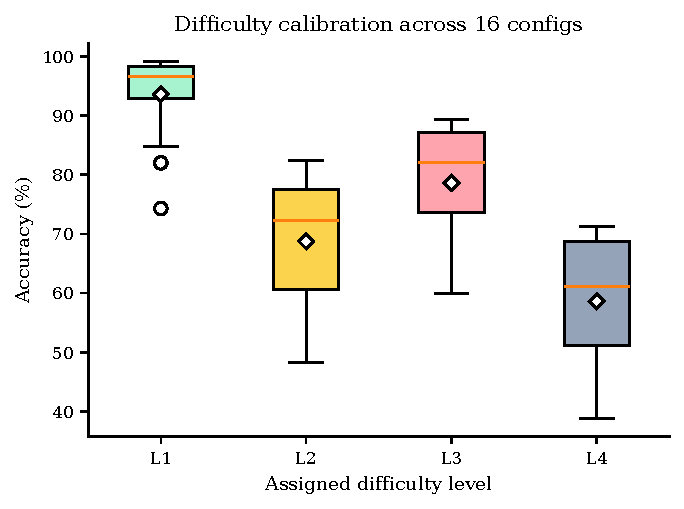
\includegraphics[width=0.65\linewidth]{figures/fig_difficulty_calib.pdf}
  \caption{Difficulty calibration: distribution of accuracy across the
    16 configs at each level. The medians sit at L1 96\%, L2 70\%, L3
    81\%, L4 60\%. The L2$<$L3 inversion is an artifact of the C4
    re-label: many questions originally tagged L2 by their generator
    were promoted to L3, leaving the residual L2 set comprising
    items that were correctly tagged in the first place — a
    smaller-but-truer L2 partition.}
  \label{fig:difficulty-box}
\end{figure}

\begin{table}[h]
  \centering
  \footnotesize
  \caption{Cost ledger and cost-per-correct-answer.}
  \label{tab:cost-ledger}
  \begin{tabular}{lrrr}
    \toprule
    Config & Total cost & Correct ans. & Cost / correct \\
    \midrule
    llama-3.1-8b               & \$0.01 & 1{,}976 & \$0.0000 \\
    llama-3.3-70b              & \$0.04 & 2{,}190 & \$0.0000 \\
    gemini-2.5-flash           & \$0.12 & 2{,}454 & \$0.0000 \\
    deepseek-v3                & \$0.12 & 2{,}295 & \$0.0001 \\
    qwen-2.5-7b                & \$0.12 & 1{,}860 & \$0.0001 \\
    qwen-2.5-72b               & \$0.15 & 2{,}202 & \$0.0001 \\
    claude-haiku-4.5           & \$0.44 & 1{,}741 & \$0.0003 \\
    mistral-large-2411         & \$0.87 & 2{,}256 & \$0.0004 \\
    gpt-5-mini                 & \$2.82 & 2{,}561 & \$0.0011 \\
    claude-opus-4.7            & \$3.35 & 2{,}647 & \$0.0013 \\
    claude-opus-4.7-thinking   & \$3.53 & 2{,}645 & \$0.0013 \\
    deepseek-r1                & \$10.54 & 2{,}517 & \$0.0042 \\
    o3                         & \$11.80 & 2{,}729 & \$0.0043 \\
    gemini-2.5-pro-thinking    & \$13.06 & 2{,}698 & \$0.0048 \\
    gpt-5                      & \$21.90 & 2{,}704 & \$0.0081 \\
    gemini-2.5-pro             & \$29.47 & 2{,}669 & \$0.0110 \\
    \bottomrule
  \end{tabular}
\end{table}

\subsection{Item analysis}

\begin{figure}[h]
  \centering
  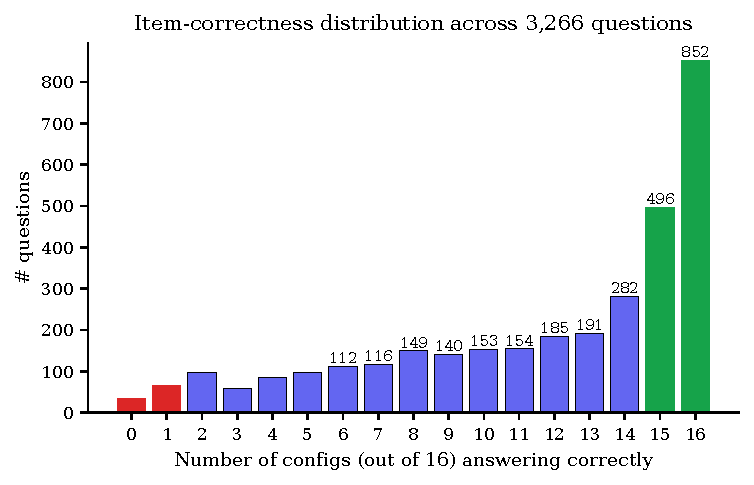
\includegraphics[width=0.75\linewidth]{figures/fig_item_histogram.pdf}
  \caption{Item-correctness distribution. The right tail (k$\geq$15
    correct) holds 1{,}348 ceiling items (41\%); the left tail
    (k$\leq$1) holds 99 items, 97 of which were audited post-eval.
    The bulk of the mass sits in the discriminating middle (k=4--14).}
  \label{fig:item-histogram}
\end{figure}

\begin{figure}[h]
  \centering
  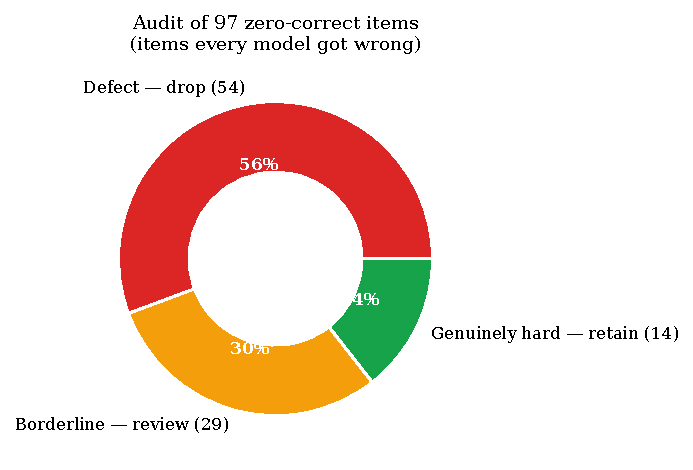
\includegraphics[width=0.5\linewidth]{figures/fig_zero_correct_donut.pdf}
  \caption{Audit of 97 zero-correct items. We reviewed all 97
    questions every model answered incorrectly: 54 were genuine corpus
    defects (wrong key, all-correct options, duplicate or equivalent
    options), 29 were borderline cases that warranted further review
    (and were dropped after a second-pass review on 2026-05-04), and
    14 were retained as legitimately hard. The defect rate (56\%
    among zero-correct items) underlines the value of an empirical
    post-eval audit alongside automated agents.}
  \label{fig:zero-correct}
\end{figure}

\subsection{Self-preference bootstrap CIs}

\begin{table}[h]
  \centering
  \footnotesize
  \caption{Per-config Self-Preference Score with 95\% bootstrap CI
    (1{,}000 resamples). DeepSeek and Mistral have no own-family
    questions in \texttt{release\_v1.2} and are omitted.}
  \label{tab:sps-full}
  \begin{tabular}{llrrrr}
    \toprule
    Config & Family & own (\%) & other (\%) & $\delta$ (pp) & 95\% CI \\
    \midrule
    claude-haiku-4.5             & anthropic & 58.8 & 48.8 & $+10.0$ & [$+5.7$, $+14.5$] \\
    claude-opus-4.7              & anthropic & 86.6 & 77.5 & $+9.1$  & [$+6.1$, $+12.1$] \\
    claude-opus-4.7-thinking     & anthropic & 86.9 & 77.2 & $+9.7$  & [$+6.5$, $+13.1$] \\
    qwen-2.5-7b                  & qwen      & 60.9 & 51.9 & $+9.0$  & [$+4.5$, $+13.2$] \\
    qwen-2.5-72b                 & qwen      & 66.1 & 64.1 & $+2.0$  & [$-2.1$, $+6.0$] \\
    llama-3.3-70b                & meta      & 65.5 & 63.6 & $+1.9$  & [$-2.3$, $+6.1$] \\
    gpt-5-mini                   & openai    & 77.9 & 76.1 & $+1.7$  & [$-2.4$, $+5.4$] \\
    o3                           & openai    & 81.9 & 82.1 & $-0.1$  & [$-3.9$, $+3.3$] \\
    gpt-5                        & openai    & 79.7 & 81.4 & $-1.7$  & [$-5.4$, $+2.1$] \\
    llama-3.1-8b                 & meta      & 54.2 & 57.2 & $-3.0$  & [$-7.3$, $+1.4$] \\
    gemini-2.5-pro               & google    & 75.0 & 81.1 & $-6.1$  & [$-10.7$, $-1.8$] \\
    gemini-2.5-pro-thinking      & google    & 74.0 & 82.0 & $-8.0$  & [$-12.3$, $-3.8$] \\
    gemini-2.5-flash             & google    & 64.3 & 74.7 & $-10.4$ & [$-15.3$, $-5.6$] \\
    \bottomrule
  \end{tabular}
\end{table}
